%% LyX 2.2.3 created this file.  For more info, see http://www.lyx.org/.
%% Do not edit unless you really know what you are doing.
\documentclass[english,12pt]{article}
\usepackage[T1]{fontenc}
\usepackage[latin9]{inputenc}
\usepackage{float}
\usepackage{mathtools}
\usepackage{amsmath}
\usepackage{amsthm}
\usepackage{amssymb}
\usepackage{graphicx}

\makeatletter
%%%%%%%%%%%%%%%%%%%%%%%%%%%%%% Textclass specific LaTeX commands.
\theoremstyle{plain}
\newtheorem{thm}{\protect\theoremname}[section]
\theoremstyle{plain}
\newtheorem{prop}[thm]{\protect\propositionname}
\ifx\proof\undefined
\newenvironment{proof}[1][\protect\proofname]{\par
\normalfont\topsep6\p@\@plus6\p@\relax
\trivlist
\itemindent\parindent
\item[\hskip\labelsep\scshape #1]\ignorespaces
}{%
\endtrivlist\@endpefalse
}
\providecommand{\proofname}{Proof}
\fi
\theoremstyle{plain}
\newtheorem{cor}[thm]{\protect\corollaryname}
\theoremstyle{definition}
\newtheorem{example}[thm]{\protect\examplename}
\theoremstyle{definition}
\newtheorem{defn}[thm]{\protect\definitionname}

%%%%%%%%%%%%%%%%%%%%%%%%%%%%%% User specified LaTeX commands.
\usepackage[margin=1in]{geometry}

\makeatother

\usepackage{babel}
\providecommand{\corollaryname}{Corollary}
\providecommand{\definitionname}{Definition}
\providecommand{\examplename}{Example}
\providecommand{\propositionname}{Proposition}
\providecommand{\theoremname}{Theorem}

\begin{document}

\title{Math 525: Lecture 8}

\date{January 30, 2018}
\maketitle

\section{Moment inequalities}

There are a few useful inequalities concerning moments of random variables
we should cover. We start with Markov's inequality.

\subsection{Markov's inequality}

The following inequality is a special case of a more general measure
theoretic result. In the measure theoretic setting, it is called Chebyshev's
inequality.
\begin{prop}[Markov's inequality]
Let $p>0$, $\lambda>0$, and $X$ be a random variable with $X^{p}$
integrable. Then,
\[
\mathbb{P}(\left\{ \left|X\right|\geq\lambda\right\} )\leq\frac{1}{\lambda^{p}}\mathbb{E}\left[\left|X\right|^{p}\right].
\]
\end{prop}
\begin{proof}
First, note that 
\[
\mathbb{P}(\left\{ \left|X\right|\geq\lambda\right\} )=\mathbb{P}(\left\{ \left|X\right|^{p}\geq\lambda^{p}\right\} )=\mathbb{E}\left[I_{\left\{ \left|X\right|^{p}\geq\lambda^{p}\right\} }\right].
\]
But if $|X(\omega)|^{p}\geq\lambda^{p}$, then $1\leq|X(\omega)|^{p}/\lambda^{p}$.
Therefore,
\[
\mathbb{E}\left[I_{\left\{ \left|X\right|^{p}\geq\lambda^{p}\right\} }\right]\leq\mathbb{E}\left[\frac{\left|X\right|^{p}}{\lambda^{p}}I_{\left\{ \left|X\right|^{p}\geq\lambda^{p}\right\} }\right]\leq\frac{1}{\lambda^{p}}\mathbb{E}\left[\left|X\right|^{p}I_{\left\{ \left|X\right|^{p}\geq\lambda^{p}\right\} }\right]\leq\frac{1}{\lambda^{p}}\mathbb{E}\left[\left|X\right|^{p}\right].\qedhere
\]
\end{proof}
\begin{cor}
Let $\lambda>0$ and $Y$ be a square integrable (i.e., $Y^{2}$ is
integrable) random variable. Then,
\[
\mathbb{P}(\left\{ \left|Y-\mathbb{E}Y\right|\geq\lambda\right\} )\leq\frac{1}{\lambda^{2}}\operatorname{Var}(Y).
\]
\end{cor}
\begin{proof}
Take $p=2$ and $X=Y-\mathbb{E}Y$ in Markov's inequality.
\end{proof}

\subsection{Cauchy-Schwarz(-Buniakovski) inequality}
\begin{prop}[Cauchy-Schwarz(-Buniakovski) inequality]
Let $X$ and $Y$ be square integrable random variables. Then,
\[
\mathbb{E}\left[XY\right]\leq\sqrt{\mathbb{E}\left[X^{2}\right]\mathbb{E}\left[Y^{2}\right]}.
\]
\end{prop}
\begin{proof}
If either $X$ or $Y$ is zero a.s., then the inequality is trivial.
Therefore, suppose that neither is zero a.s. Let $\lambda\geq0$.
Then,
\[
0\leq\mathbb{E}\left[\left(X-\lambda Y\right)^{2}\right]=\mathbb{E}\left[X^{2}\right]-2\lambda\mathbb{E}\left[XY\right]+\lambda^{2}\mathbb{E}\left[Y^{2}\right]
\]
and hence
\[
\mathbb{E}\left[XY\right]\leq\frac{1}{2}\left(\frac{1}{\lambda}\mathbb{E}\left[X^{2}\right]+\lambda\mathbb{E}\left[Y^{2}\right]\right).
\]
Letting $\lambda=\sqrt{\mathbb{E}\left[X^{2}\right]}/\sqrt{\mathbb{E}\left[Y^{2}\right]}$
yieldsw
\begin{align*}
\mathbb{E}\left[XY\right] & \leq\frac{1}{2}\left(\frac{\sqrt{\mathbb{E}\left[Y^{2}\right]}}{\sqrt{\mathbb{E}\left[X^{2}\right]}}\mathbb{E}\left[X^{2}\right]+\frac{\sqrt{\mathbb{E}\left[X^{2}\right]}}{\sqrt{\mathbb{E}\left[Y^{2}\right]}}\mathbb{E}\left[Y^{2}\right]\right)\\
 & =\frac{\mathbb{E}\left[Y^{2}\right]\mathbb{E}\left[X^{2}\right]}{\sqrt{\mathbb{E}\left[X^{2}\right]\mathbb{E}\left[Y^{2}\right]}}\\
 & =\sqrt{\mathbb{E}\left[X^{2}\right]\mathbb{E}\left[Y^{2}\right]}.\qedhere
\end{align*}
\end{proof}
\begin{example}
Let $X\sim\operatorname{Poisson}(\lambda)$ and $Y\sim\operatorname{Bernoulli}(p)$
be random variables. Then, by the Cauchy-Schwarz inequality,
\[
\mathbb{E}\left[XY\right]\leq\sqrt{\mathbb{E}\left[X^{2}\right]\mathbb{E}\left[Y^{2}\right]}=\sqrt{\lambda\left(\lambda+1\right)p}.
\]
If the two random variables are independent, then
\[
\mathbb{E}\left[XY\right]=\mathbb{E}X\mathbb{E}Y=\lambda p.
\]
Indeed, you can check that for all $0\leq p\leq1$ and $\lambda\geq0$,
\[
\lambda p\leq\sqrt{\lambda\left(\lambda+1\right)p}.
\]
\end{example}

\section{Jensen's inequality}

Next, we will cover Jensen's inequality, probably one of the most
useful inequalities in probability theory! To discuss Jensen's inequality,
we need to recall the notion of a convex function:
\begin{defn}
Let $X$ be a subset of $\mathbb{R}^{n}$. We say $X$ is \emph{convex}
if for all points $x,y\in X$ and $\theta\in[0,1]$, we have $\theta x+(1-\theta)y\in X$.
\end{defn}
\begin{figure}
\begin{centering}
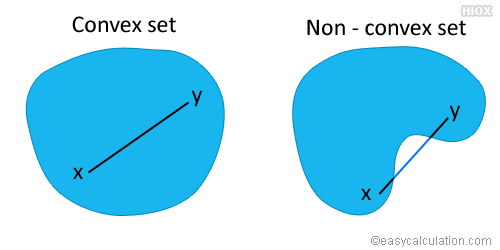
\includegraphics[width=4in]{convex}
\par\end{centering}
\caption{Examples of convex and non-convex sets}
\end{figure}
\begin{defn}
Let $X$ be convex and $f\colon X\rightarrow\mathbb{R}$. We call
the set
\[
\operatorname{epi}(f)=\left\{ (x,\mu)\in X\times\mathbb{R}\colon f(x)\leq\mu\right\} 
\]
the \emph{epigraph} of $f$. We say $f$ is a \emph{convex function
}if its epigraph is convex. We say $f$ is \emph{concave} if $-f$
is convex.
\end{defn}
Intuitively, a convex function is one whose epigraph makes a ``bowl'':

\begin{figure}
\begin{centering}
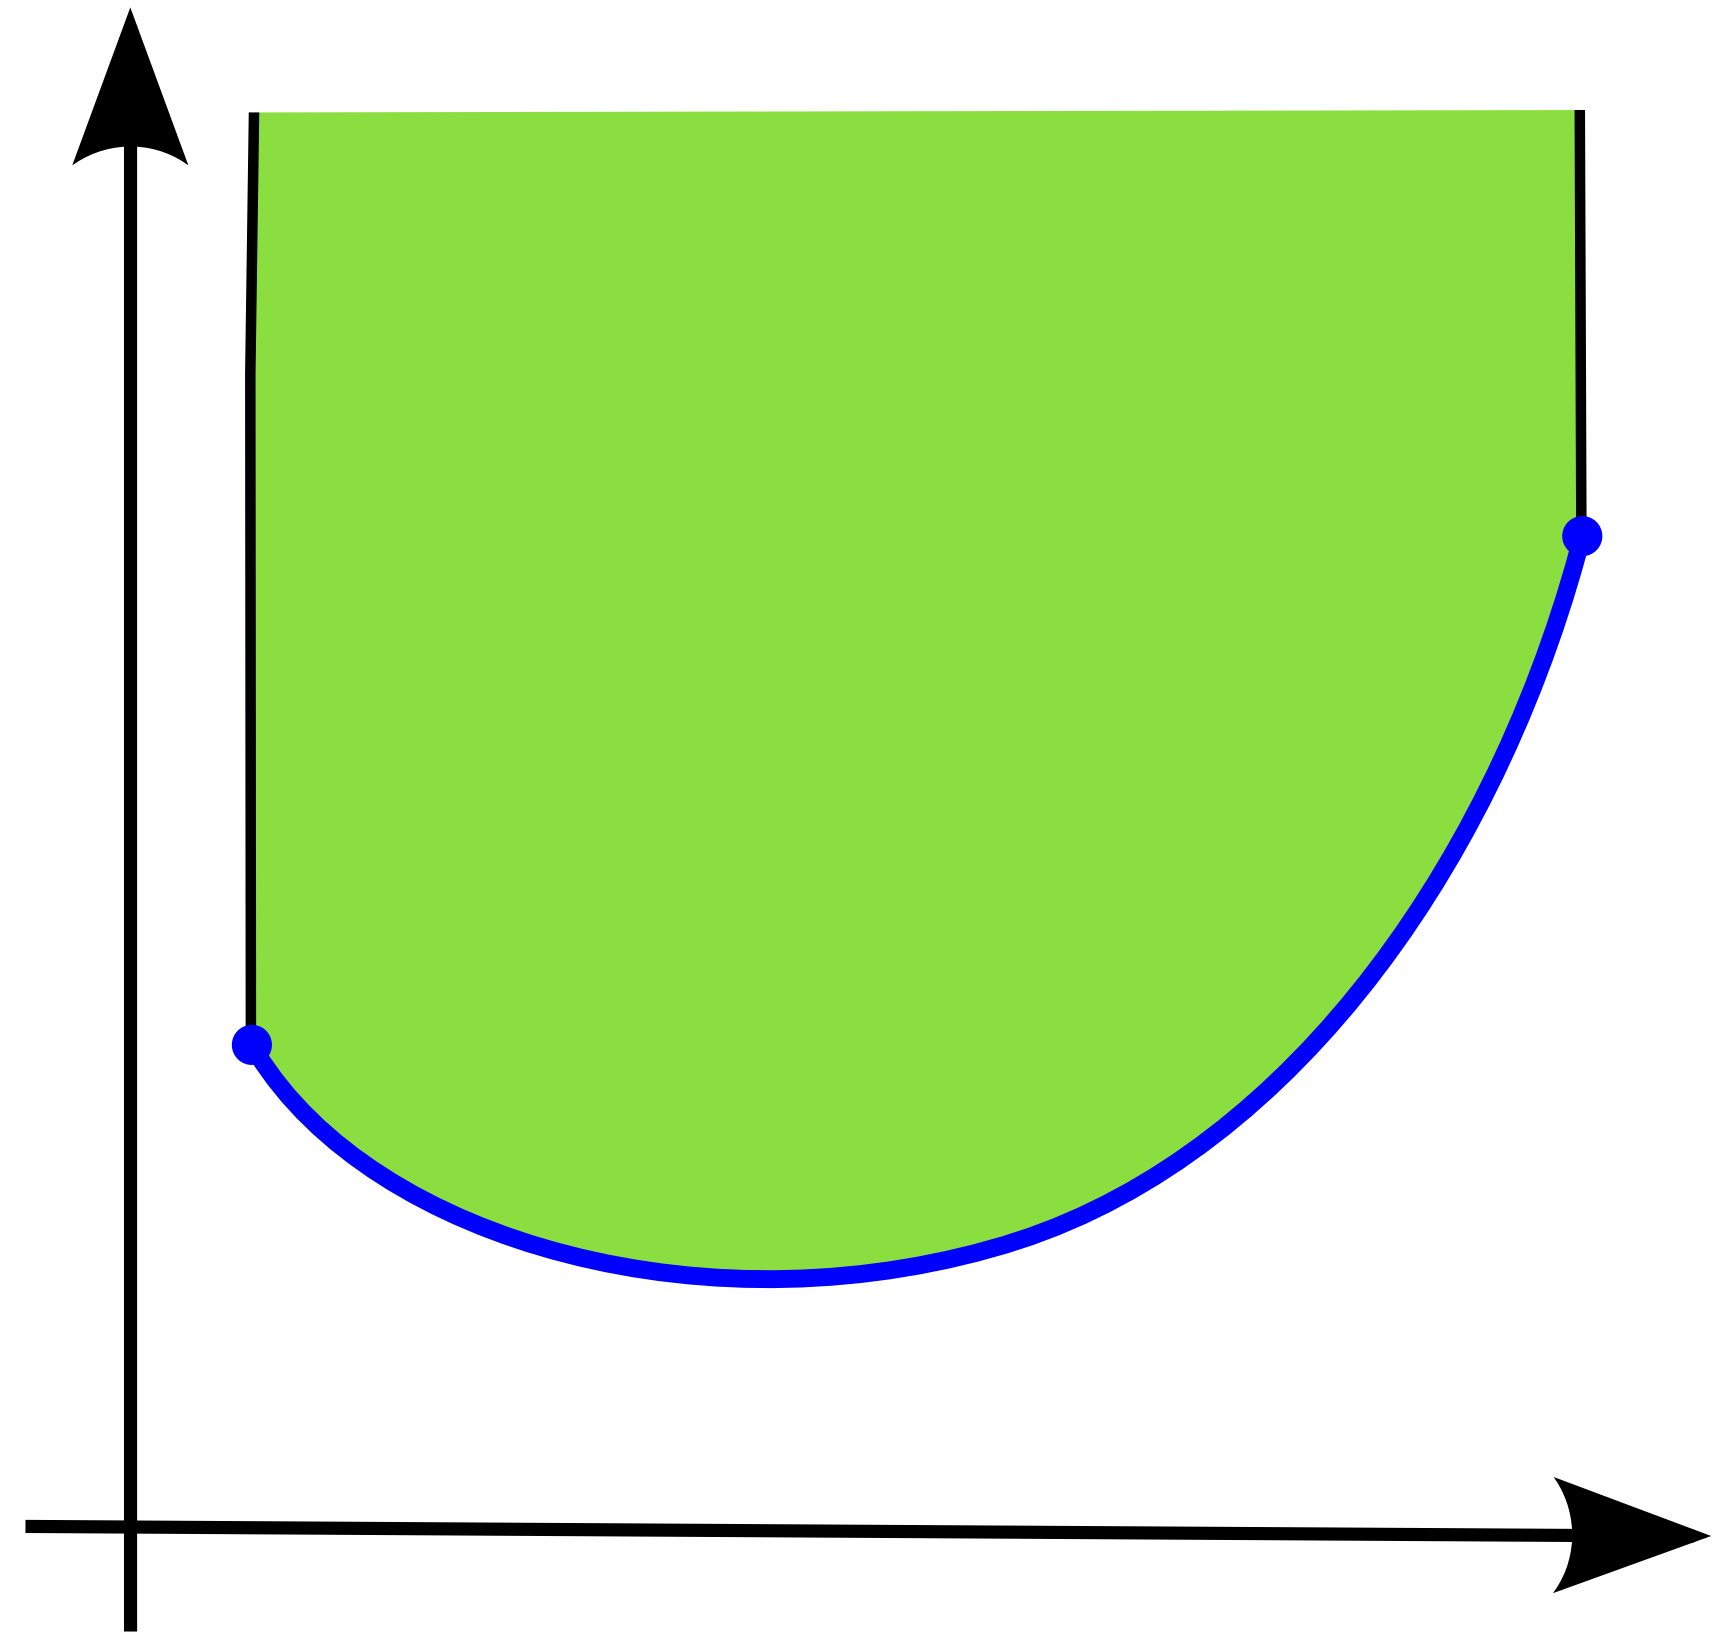
\includegraphics[width=4in]{epigraph}
\par\end{centering}
\caption{Epigraph (green) of a function $f$ (blue curve)}
\end{figure}
\begin{example}
$x$, $|x|$, $x^{2}$, $e^{-x}$ are convex on $\mathbb{R}$. The
function $f$ defined by
\[
f(x)=\begin{cases}
1/x & \text{if }x\neq0\\
0 & \text{if }x=0
\end{cases}
\]
is not convex on $\mathbb{R}$, but it is convex on $(-\infty,0)$
and $(0,\infty)$.
\end{example}
\begin{prop}
Let $X$ be convex and $f\colon X\rightarrow\mathbb{R}$. $f$ is
\emph{a }convex function if and only if for all $x,y\in X$ and $\theta\in[0,1]$,
\[
f(\theta x+\left(1-\theta\right)y)\leq\theta f(x)+\left(1-\theta\right)f(y).
\]
\end{prop}
\begin{proof}
Suppose $f$ is a convex function. Let $x,y\in X$ and $\theta\in[0,1]$.
Note that $(x,f(x))$ and $(y,f(y))$ are both points in $\operatorname{epi}(f)$.
By convexity,
\[
\theta(x,f(x))+(1-\theta)(y,f(y))=(\theta x+\left(1-\theta\right)y,\theta f(x)+\left(1-\theta\right)f(y))\in\operatorname{epi}(f)
\]
and hence 
\[
f(\theta x+\left(1-\theta\right)y)\leq\theta f(x)+\left(1-\theta\right)f(y),
\]
as desired.

Suppose $f$ satisfies the convexity inequality. Let $(x,\mu_{x})$
and $(y,\mu_{y})$ be points in $\operatorname{epi}(f)$ and $\theta\in[0,1]$.
By the convexity inequality,
\[
f(\theta x+\left(1-\theta\right)y)\leq\theta f(x)+\left(1-\theta\right)f(y)\leq\theta\mu_{x}+\left(1-\theta\right)\mu_{y}
\]
and hence 
\[
\theta(x,\mu_{x})+\left(1-\theta\right)(y,\mu_{y})=(\theta x+\left(1-\theta\right)y,\theta\mu_{x}+\left(1-\theta\right)\mu_{y})\in\operatorname{epi}(f),
\]
as desired.
\end{proof}
%
\begin{prop}
A convex set in $\mathbb{R}$ is an interval.
\end{prop}
\begin{proof}
Suppose $X\subset\mathbb{R}$ is convex and not an interval. Let $x,z\in X$
and $y$ be such that $x<y<z$. Pick 
\[
\theta=\frac{z-y}{z-x}.
\]
Then,
\[
\theta x+\left(1-\theta\right)y=\frac{z-y}{z-x}x+\frac{y-x}{z-x}z=\frac{xz-xy}{z-x}+\frac{yz-xz}{z-x}=\frac{yz-xy}{z-x}=y.
\]
\end{proof}
\begin{prop}
\label{prop:alternate_characterization}Let $I$ be an interval and
$f\colon I\rightarrow\mathbb{R}$. Then, $f$ is convex if and only
if for all points $x,y,x^{\prime},y^{\prime}\in I$ such that $x\leq x^{\prime}<y^{\prime}$
and $x<y\leq y^{\prime}$,
\[
\frac{f(y)-f(x)}{y-x}\leq\frac{f(y^{\prime})-f(x^{\prime})}{y^{\prime}-x^{\prime}}.
\]
\end{prop}
\begin{proof}
Suppose $f$ is convex and let $A=(x,f(x))$, $B=(y,f(y))$, $C=(x^{\prime},f(x^{\prime}))$,
and $D=(y^{\prime},f(y^{\prime}))$. Then... (proof by picture)

\begin{figure}[H]
\centering{}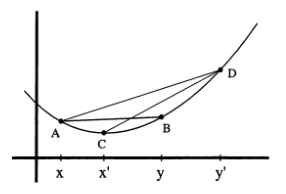
\includegraphics{chords}
\end{figure}

For the converse, let $x_{1},x_{2}\in I$ and $\theta\in[0,1]$. Take
$x=x_{1}$, $y^{\prime}=x_{2}$, and $y=x^{\prime}=\theta x_{1}+(1-\theta)x_{2}$
to get
\[
\frac{f(\theta x_{1}+(1-\theta)x_{2})-f(x_{1})}{\theta x_{1}+(1-\theta)x_{2}-x_{1}}\leq\frac{f(x_{2})-f(\theta x_{1}+(1-\theta)x_{2})}{x_{2}-\theta x_{1}-(1-\theta)x_{2}}
\]
and hence
\[
\theta\left(f(\theta x_{1}+(1-\theta)x_{2})-f(x_{1})\right)\left(x_{2}-x_{1}\right)\leq\left(1-\theta\right)\left(f(x_{2})-f(\theta x_{1}+(1-\theta)x_{2})\right)\left(x_{2}-x_{1}\right).
\]
Simplifying,
\[
f(\theta x_{1}+(1-\theta)x_{2})\leq\theta f(x_{1})+\left(1-\theta\right)f(x_{2}).\qedhere
\]
\end{proof}
\begin{cor}
Let $I=(a,b)$ be an open interval and $f\colon I\rightarrow\mathbb{R}$
be a convex function. Then, $f$ is continuous and the left and right
derivatives 
\[
D_{-}f(x)=\lim_{h\downarrow0}\frac{f(x)-f(x-h)}{h}\qquad\text{and}\qquad D_{+}f(x)=\lim_{h\downarrow0}\frac{f(x+h)-f(x)}{h}
\]
exist at each point $x\in I$. Moreover, $D_{-}$f and $D_{+}f$ are
nondecreasing with $D_{-}f\leq D_{+}f.$
\end{cor}
\begin{proof}
Let $x$ be a point in $I$. By Proposition \ref{prop:alternate_characterization},
for all $h>0$ such that $x-h$ and $x+h$ are points in $I$,
\begin{equation}
\frac{f(x)-f(x-h)}{h}\leq\frac{f(x+h)-f(x)}{h}.\label{eq:inequality}
\end{equation}
We would like to take limits and conclude
\[
D_{-}f(x)=\lim_{h\downarrow0}\frac{f(x)-f(x-h)}{h}\leq\lim_{h\downarrow0}\frac{f(x+h)-f(x)}{h}=D_{+}f(x).
\]
But first, we have to show these limits exist: note that Proposition
\ref{prop:alternate_characterization} implies that the left hand
side of (\ref{eq:inequality}) increases while the right hand side
of (\ref{eq:inequality}) decreases as $h$ is made smaller. That
is, for a decreasing sequence of $(h_{n})_{n}$ with $h_{n}\downarrow0$,
\[
\frac{f(x)-f(x-h_{1})}{h}\leq\frac{f(x)-f(x-h_{2})}{h}\leq\cdots\leq\frac{f(x+h_{2})-f(x)}{h}\leq\frac{f(x+h_{1})-f(x)}{h}.
\]
Then, the limits exist by the monotone convergence theorem (recall
that the monotone convergence theorem for sequences says that if a
sequence is nondecreasing and bounded above, it must have a limit).
\end{proof}
\begin{prop}
Let $I=(a,b)$ be an open interval and $f\colon I\rightarrow\mathbb{R}$
be a convex function. Then, for each $x_{0}\in I$, there exists $m$
such that for all $x\in I$,
\[
f(x)\geq f(x_{0})+m\left(x-x_{0}\right).
\]
That is, at each point $x_{0}$, there exists a \textbf{supporting
line}.
\end{prop}
This fact generalizes to higher dimensions, in which case the supporting
line becomes a \textbf{supporting hyperplane}.
\begin{proof}
Choose $m$ such that
\[
D_{-}f(x_{0})\leq m\leq D_{+}f(x_{0}).
\]
Now, if $x>x_{0}$,
\[
m\leq D_{+}f(x_{0})=\lim_{h\downarrow0}\frac{f(x_{0}+h)-f(x_{0})}{h}\leq\frac{f(x)-f(x_{0})}{x-x_{0}}
\]
and hence
\[
f(x_{0})+m\left(x-x_{0}\right)\leq f(x).
\]
The case of $x<x_{0}$ is identical (use $D_{-}f(x_{0})$ in the argument).
\end{proof}
\begin{prop}[Jensen's inequality]
Let $I=(a,b)$ be an open interval and $f\colon I\rightarrow\mathbb{R}$
be a convex function. Let $X$ be a random variable which takes values
in $(a,b)$ a.s. If $X$ and $f\circ X$ are both integrable,
\[
\mathbb{E}\left[f(X)\right]\geq f(\mathbb{E}X).
\]
\end{prop}
\begin{proof}
Let $x_{0}=\mathbb{E}X$. Now, we can find some supporting line parameterized
by $m$:
\[
f(x)\geq f(x_{0})+m(x-x_{0}).
\]
Substitute $x=X$ to get
\[
f(X)\geq f(x_{0})+m(X-x_{0})
\]
(this inequality holds only a.s.). Take expectations of both sides
to get
\[
\mathbb{E}\left[f(X)\right]\geq\mathbb{E}\left[f(x_{0})+m(X-x_{0})\right]=\mathbb{E}\left[f(x_{0})\right]=f(x_{0})=f(\mathbb{E}X).\qedhere
\]
\end{proof}

\end{document}
